\section{Resultados}
\subsection{Experimentacion con Imagenes Reducidas}
\subsubsection{Metodo 0: Utilizando $A^tA$}
\textbf{Mediciones de TK}

\begin{figure}[H]
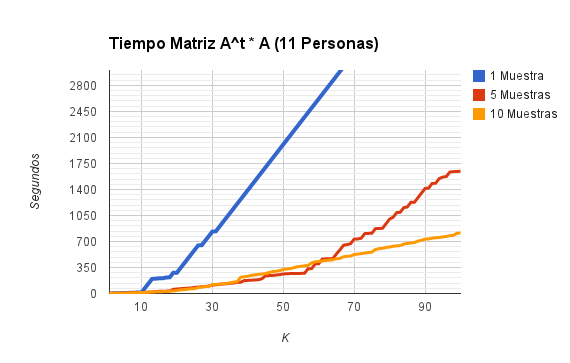
\includegraphics[width=1\textwidth]{img/image1.png}
     \caption{Tiempos Matrix $A^tA$ con 11 personas variando K}
     \label{fig:figura1}
\end{figure}

\begin{figure}[H]
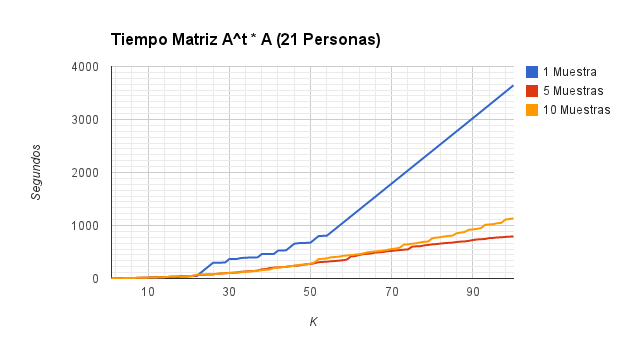
\includegraphics[width=1\textwidth]{img/image2.png}
     \caption{Tiempos Matrix $A^tA$ con 21 personas variando K}
     \label{fig:figura1}
\end{figure}


\begin{figure}[H]
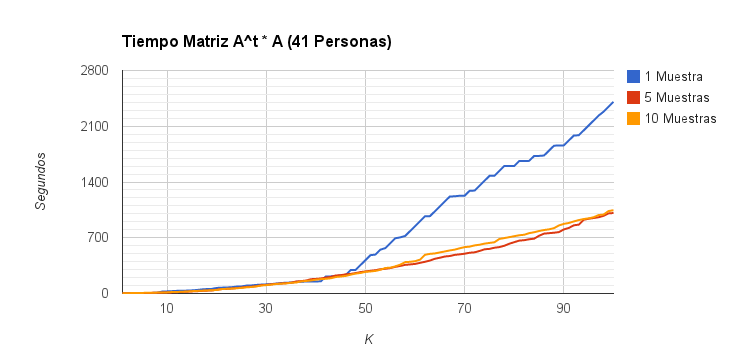
\includegraphics[width=1\textwidth]{img/image3.png}
     \caption{Tiempos Matrix $A^tA$ con 41 personas variando K}
     \label{fig:figura1}
\end{figure}




\subsubsection{Metodo 1: Utilizando $AA^t$}
\subsection{Experimentacion con Imagenes Full}
\subsubsection{Metodo 0: Utilizando $A^tA$}
\subsubsection{Metodo 1: Utilizando $AA^t$}